\section{Header instance.h}
\begin{frame}[fragile, shrink=10]{Header instance.h - Define}
  Sono state aggiunte le seguenti define nel file instance.h

  \begin{block}{\lstinline[language=C]!#define NUM_AUTORNG_RNG M/2!}
  Definisce il numero $M$ di misure raccolte durante l'autoranging da ogni ancora master per ogni range di interesse.\\
  \textcolor{dgreen}{esempio:} A0 raccoglie $M$ misure di $r_{01}$, $M$ misure di $r_{02}$ ed $M$ misure di $r_{03}$.
  \end{block}

  \begin{block}{\lstinline[language=C]!#define AUTORANGING_MAX_TIMEOUT_TAG ...!}
  Tempo in \SI{}{\milli\second} dopo il quale il tag inizia la normale procedura di ranging se non
  riceve più messaggi di POLL inviati da un'ancora master.
  \end{block}

  \begin{block}{\lstinline[language=C]!#define  ANCH_FINAL_MSG_LEN 34!}
    Lunghezza del messaggio di tipo \lstinline[language=C]!RTLS_DEMO_MSG_ANCH_FINAL!.\\
    Essa è pari a quella del messaggio di tipo \lstinline[language=C]!RTLS_DEMO_MSG_TAG_FINAL! più uno dato
    che contiene un byte in più che serve ad indicare alle ancore che l'autoranging per la corrente
    ancora master è terminato.
  \end{block}
\end{frame}

\begin{frame}[fragile]{Header instance.h - Define}
  \begin{block}{\lstinline[language=C]!#define NUM_ALL_AUTORANING_RANGES!}
  Numero complessivo di range che il tag si aspetta di ricevere da tutte le ancore.\\
  Scritto in funzione del numero totale di ancore $N$.\\
  \textcolor{dgreen}{esempio:} per $4$ ancore
  \[
  |\{r_{01}, r_{02}, r_{03}, r_{12}, r_{13}, r_{23}\}| = 3 + 2 + 1 = 6
  \]
  \alert{in generale:}
  \[
  \frac{(N-1) (N-1+1)}{2} = \frac{(N-1)N}{2}
  \]
  \end{block}
\end{frame}

\begin{frame}[fragile]{Header instance.h - Define}
  \begin{block}{\lstinline[language=C]!#define END_AUTORANGING 33!}
    Posizione, all'interno di \lstinline[language=C]!instance_data[0].msg_f.messageData!, del byte
    che indica la fine della procedura di autoranging per una data ancora master.\\
    In questo caso messageData contiene un messaggio di tipo \lstinline[language=C]!RTLS_DEMO_MSG_ANCH_FINAL!.
  \end{block}
  \begin{block}{\lstinline[language=C]!#define AUTORANGING_RANGES 8!}
    Posizione, all'interno di \lstinline[language=C]!instance_data[0].msg_f.messageData!, a partire dalla quale
    l'ancora inserisce le medie dei range che le competono.\\
    In questo caso messageData contiene un messaggio di tipo \lstinline[language=C]!RTLS_DEMO_MSG_ANCH_RESP!.
  \end{block}
\end{frame}

\begin{frame}[fragile]{Header instance.h - Struct \lstinline[language=C]!sfConfig_t!}
  Le seguenti \lstinline[language=C]!struct! sono state modificate
  \begin{C}
    typedef struct
    {
      ...
      uint16 tagPollSleepDly;
      uint16 anchPollSleepDly;
      ...
    } sfConfig_t;
  \end{C}
  È stato aggiunto il campo \lstinline[language=C]!anchPollSleepDly! e il campo \lstinline[language=C]!pollSleepDly! è stato rinominato
  \lstinline[language=C]!tagPollSleepDly! per maggiore chiarezza.\\
  Il campo \lstinline[language=C]!anchPollSleepDly! rappresenta il periodo in \SI{}{\milli\second} di trasmissione dei Poll
  dell'ancora master.

\end{frame}

\begin{frame}[fragile]{Header instance.h - Struct \lstinline[language=C]!instance_data_t!}
  \begin{C}
    typedef struct
    {
      ...
    } instance_data_t;
  \end{C}
  Sono stati aggiunti i seguenti campi
  \begin{block}{\lstinline[language=C]!int32 anchSleepTime_ms!}
    Periodo in \SI{}{\milli\second} di trasmissione dei Poll dell'ancora master
  \end{block}
  
  \begin{block}{\lstinline[language=C]!unsigned long autoranging_poll_time!}
    Se il dispositivo si comporta come ancora in modalità \lstinline[language=C]!ANCHOR_RNG! ed è l'ancora master
    rappresenta l'istante di tempo, secondo l'orologio interno, in cui è stato spedito l'ultimo Poll.\\
    Utilizzato per capire se sono passati \lstinline[language=C]!anchSleepTime_ms! \SI{}{\milli\second} dall'invio dell'ultimo Poll.
  \end{block}
\end{frame}

\begin{frame}{Header instance.h - Struct \lstinline[language=C]!instance_data_t!}
  \begin{block}{\lstinline[language=C]!unsigned long autoranging_poll_time! - continuazione}
    Se invece il dispositivo si comporta come tag in modalità \lstinline[language=C]!TAG_WAIT! rappresenta l'istante di tempo, secondo l'orologio
    interno, in cui il tag ha ricevuto l'ultimo Poll inviato da un'ancora master.\\
    Utilizzato per capire se sono passati \lstinline[language=C]!AUTORANGING_MAX_TIMEOUT_TAG! \SI{}{\milli\second} dalla ricezione
    dell'ultimo Poll inviato da un'ancora master.
  \end{block}
  \begin{block}{\lstinline[language=C]!uint8 autoranging_timeout!}
    Abilitazione del timer usato da un'ancora master per inviare periodicamente Poll alle altre ancore.\\
    Abilitazione del timer usato da un tag in modalità \lstinline[language=C]!TAG_WAIT! per attendere la fine della
    procedura di autoranging.
  \end{block}
\end{frame}

\begin{frame}{Header instance.h - Struct \lstinline[language=C]!instance_data_t!}
  \begin{block}{\lstinline[language=C]!double anchRngArray[MAX_ANCHOR_LIST_SIZE]!}
    Contiene la somma dei range raccolti da una data ancora.\\
    \textcolor{dgreen}{esempio:} sia l'ancora A1. \lstinline[language=C]!anchrRngArray[0]! contiene la somma dei range $r_{01}$,
    \lstinline[language=C]!anchrRngArray[2]! contiene la somma dei range $r_{12}$ e \lstinline[language=C]!anchrRngArray[3]! contiene la somma dei range $r_{13}$.
  \end{block}
  \begin{block}{\lstinline[language=C]!uint16 anchRngArrayCounter!}
    Contiene il numero di misure raccolte per ciascun range di interesse per una data ancora.\\
    \textcolor{dgreen}{esempio:} sia l'ancora A1. \lstinline[language=C]!anchrRngArrayCounter[0]! contiene il numero di misure del range $r_{01}$,
    \lstinline[language=C]!anchrRngArrayCounter[2]! contiene il numero di misure del range $r_{12}$ e \lstinline[language=C]!anchrRngArrayCounter[3]! contiene il numero di misure del range $r_{13}$.
  \end{block}
\end{frame}

\begin{frame}{Header instance.h - Struct \lstinline[language=C]!instance_data_t!}
  \begin{block}{\lstinline[language=C]!uint8 autoRngRangesRxMask!}
    Bitmask. Il bit i-esimo vale 1 se il tag ha ricevuto \alert{tutte} le medie dei range dall'ancora i-esima.
  \end{block}
  \begin{block}{\lstinline[language=C]!double autoRngRangesArray[NUM_ALL_AUTORANGING_RANGES]!}
    Medie dei range ricevute dal tag.\\
    \textcolor{dgreen}{esempio:} Nel caso di 4 ancore \lstinline[language=C]!autoRngRangesArray[0]! $ = r_{01}$,
    \hdots, \lstinline[language=C]!autoRngRangesArray[5]! $ = r_{23}$.
  \end{block}
  \begin{block}{\lstinline[language=C]!float anchorPositionMatrix[3 * MAX_ANCHOR_LIST_SIZE]!}
    Posizioni cartesiane delle ancore ottenute con apposito algoritmo a partire dalle medie dei range salvate
    in \lstinline[language=C]!autoRngRangesArray!.\\
    \alert{in generale:} \lstinline[language=C]!anchorPositionMatrix[i][j]! contiene la coordinata $i$-esima dell'ancora $j$-esima.
  \end{block}
\end{frame}

\begin{frame}{Header instance.h - Struct \lstinline[language=C]!instance_data_t!}
  \begin{block}{\lstinline[language=C]!uint8 tagPositionsSentToViewer!}
    Contatore utilizzato per inviare ad intervalli regolari la posizione delle ancore sulla porta seriale
    virtuale (USB OTG VCP). Tali posizioni sono utilizzate dal Viewer 3D (di cui si parlerà nel seguito).
  \end{block}
  \begin{block}{\lstinline[language=C]!uint16 anchorRngMaster!}
    Contiene l'ID corrente dell'ancora master durante l'autoranging.
  \end{block}
\end{frame}

\begin{frame}[shrink=10]{Header instance.h - Struct \lstinline[language=C]!instance_data_t! - \lstinline[language=C]!rxResponseMaskAnc!}
  Il campo \lstinline[language=C]!rxResponseMaskAnc! era già presente nella struct \lstinline[language=C]!instance_data_t!.
  \par
  Durante la procedura di autoranging l'ancora master mette ad $1$ il bit i-esimo se ha rivecuto risposta dall'ancora i-esima.
  \par
  Le ancore \alert{non} master, invece, utilizzano questo campo per decidere quando è il momento di rispondere.
  Rispetto alla normale procedura di ranging, nella quale la prima ancora a rispondere è sempre l'ancora A0, durante la
  procedura di autoranging è più complicato, per ogni ancora, decidere quando rispondere. Infatti quando l'ancora master non è A0
  l'ordine in cui le ancore devono rispondere non è scontato. Ad esempio quando A2 si comporta da ancora master l'ordine di risposta delle ancore
  dovrà essere A0, A1, A3.\\
  Per non scrivere un codice ad hoc per specificare l'ordine di risposta al variare di ogni ancora master la maschera \lstinline[language=C]!rxResponseMaskAnc!
  è stata utilizzata come spiegato nell'esempio della slide successiva.
\end{frame}

\begin{frame}[shrink=10]{Header instance.h - Struct \lstinline[language=C]!instance_data_t! - \lstinline[language=C]!rxResponseMaskAnc!}
  L'invio delle risposte da parte delle ancore viene regolato dalla maschera \lstinline[language=C]!rxResponseMaskAnc!.
  Viene mostrato un esempio in cui l'ancora A2 si comporta da master.
  \begin{columns}
    \begin{column}{0.4\textwidth}
      \begin{center}
        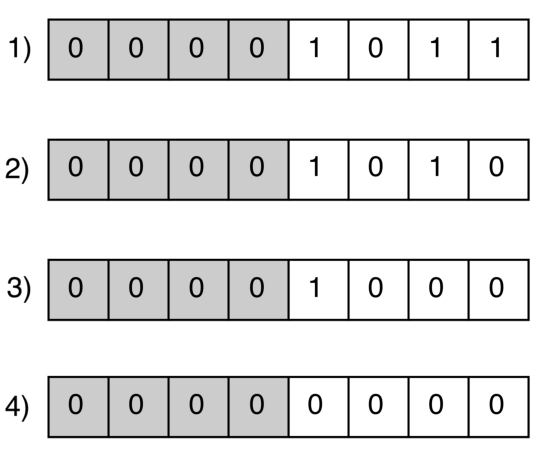
\includegraphics[width=\linewidth]{rxResponseMaskAnc.pdf}
      \end{center}
    \end{column}
    \begin{column}{0.7\textwidth}
      \begin{itemize}
      \item[1.] la maschera viene inizializzata all'arrivo del Poll in tutte le ancore mettendo a $0$ il bit corrispondente alla posizione dell'ancora master
      \item[2.] dopo che l'ancora $0$ ha risposto viene posto a $0$ il bit corrispondente alla posizione dell'ancora 
      \item[3.] dopo che l'ancora $1$ ha risposto viene posto a $0$ il bit corrispondente alla posizione dell'ancora 
      \item[4.] dopo che l'ancora $3$ ha risposto viene posto a $0$ il bit corrispondente alla posizione dell'ancora 
      \end{itemize}
    \end{column}
  \end{columns}
  \begin{exampleblock}{L'ancora i-esima decide di rispondere}
    quando è il primo bit (da destra) diverso da $0$ è il bit i-esimo.
  \end{exampleblock}
\end{frame}

\begin{frame}[fragile]{Header instance.h - Enum}
  Il seguente enum è stato modificato
  \begin{C}
    typedef enum instanceModes{LISTENER, TAG, TAG_WAIT, ANCHOR, ANCHOR_RNG, NUM_MODES} INST_MODE;
  \end{C}
  È stato aggiunto l'enumeratore \lstinline[language=C]!TAG_WAIT!. Esso corrisponde alla modalità in cui il tag
  attende il completamento della procedura di autoranging.
\end{frame}
